% -*- coding: utf-8 -*-
\documentclass[a4paper]{article}
\usepackage[utf8]{inputenc}
\usepackage[T1]{fontenc}
\usepackage[american]{babel}
\usepackage{listings}
\usepackage{hyperref}
\usepackage{makeidx}
\usepackage[totoc]{idxlayout}
\usepackage{color}
\usepackage{graphicx}
\usepackage[margin=3cm]{geometry}
\usepackage{placeins}
\usepackage{siunitx}
\usepackage{minted}  % requires -shell-escape option for latex

% minted has no stable support for inline code, so we use listings here
\lstMakeShortInline[basicstyle=\small\ttfamily]|

\lstdefinestyle{terminal}
{
  backgroundcolor=\color{white},
  basicstyle=\scriptsize\color{black}\ttfamily
}

\makeindex

\begin{document}
\title{Pyphant Manual}
\author{Alexander Held}

\maketitle

\date{}

\begin{abstract}
  This manual describes the structure and use of
  pyphant. Pyphant is an open source project
  currently developed mainly by the service group ``Scientific Data
  Processing'' at the Freiburg Materials Research Center, University
  of Freiburg, Germany. Pyphant consists of a collection of python
  packages offering a framework for scientific data analysis. It
  includes an extension of numpy's arrays offering
  support for axes and units along with a collection of building
  blocks for the development of data processing algorithms organized
  into toolboxes. Pyphant features a flexible plugin architecture
  allowing for the application in many different fields. It ships with
  a graphical user interface allowing for the development of
  scientific data analysis workflows using graphical programming.
\end{abstract}

\tableofcontents

\section{Introduction}
\label{sec:introduction}

Until this document is finished, please also see
Reference\cite{pyphant} and the source code on
github\cite{pyphanturl}.

\subsection{Installation}
\label{sec:introduction_installation}

Until this document is finished, please refer to the readme file on
github\cite{pyphanturl}.

\subsection{Pyphant Quick Tour}
\label{sec:introduction_a_quick_tour}

In this quick tour, you will learn how to use pyphant's graphical user
interface (GUI) for graphical programming and how to extend pyphant by
writing your own workers and visualizers as well as some basic
scripting with pyphant's python application programming interface
(API).

\subsubsection{Working with the graphical user interface}
\label{sec:introduction_gui}

As a first example, we want to develop a simple image processing
algorithm that calculates a histogram of the gradient magnitude of an
input image built from the processing steps available in pyphant's
|ImageProcessing| and |Statistics| toolboxes using graphical
programming. These processing steps are called workers and a specific
arrangement of workers is called a recipe. Let us begin by opening
pyphant's GUI in order to create a new recipe. This is done by passing
the filename of the recipe to the GUI script:
\begin{minted}{bash}
$ wxPyphant quicktour.h5
\end{minted}
We assume a Linux or OS X installation for this quick tour. MS Windows
users, please refer to the instructions in the readme
file\cite{wingui}. Recipes are stored in the HDF5\cite{hdf5} data
format and the file extension has to be |.h5| for that
reason. The above command should bring up pyphant's splash
screen and then a window similar to \autoref{fig:gui}.
\begin{figure}[h]
  \centering
  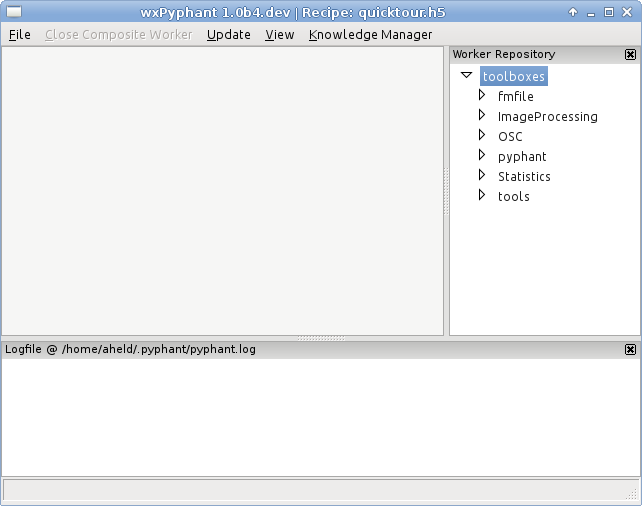
\includegraphics[scale=0.75]{fig/gui.png}
  \caption{Pyphant's graphical user interface}
  \label{fig:gui}
\end{figure}
The title bar shows pyphant's version and the recipe's filename. On
the right hand side, the installed toolboxes are listed in a tree
view. Each toolbox can be expanded to access the individual workers
contained in it. A worker can be placed on the central grey area
representing the recipe by a drag and drop operation. Let's try this
out with the |Load Image| worker from the |ImageProcessing|
toolbox. The drag and drop operation results in the worker appearing
on the central pane as depicted in \autoref{fig:gui_add_LI_worker}.
\begin{figure}[h]
  \centering
  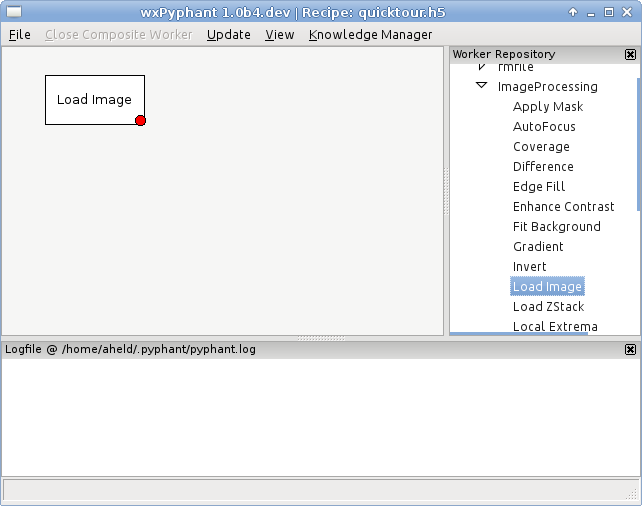
\includegraphics[scale=0.75]{fig/gui_add_LI_worker.png}
  \caption{Adding a worker to the recipe}
  \label{fig:gui_add_LI_worker}
\end{figure}
In order to be able to load an image, we have to tell pyphant about
its location. This is done by adjusting the |Filename| parameter of
the |Load Image| worker. For this purpose, simply click once onto the
worker. This brings up a dialog with all the adjustable parameters as
shown in \autoref{fig:gui_LI_worker_parameters}.
\begin{figure}[h]
  \centering
  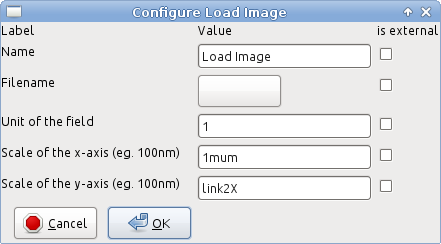
\includegraphics[scale=0.75]{fig/gui_LI_worker_parameters.png}
  \caption{Editing the parameters of a worker}
  \label{fig:gui_LI_worker_parameters}
\end{figure}
Clicking on the button to the right of the |Filename| label brings up
a file picker dialog. Use this dialog to select any image at hand.

The |Load Image| worker takes image data from a file and converts it
to pyphant's internal format. If the image has multiple color
channels, it will be converted to a gray scale image first. In our
case, the resulting internal format is a two dimensional
|FieldContainer|. In general, a |FieldContainer| is a discretized
scalar valued field with a unit for the field values and as many axes
as there are dimensions. An axis is itself a one dimensional
|FieldContainer|. The recursion is eventually ended by a sentinel
value for the dimensions. For further details also refer to
\autoref{sec:data_model} and Reference~\cite{pyphant}. As a side note
for the readers familiar with numpy\cite{numpy}, a |FieldContainer| is
an extension of a numpy array adding units, axes and some more
features. This explains the occurance of the three other parameters in
\autoref{fig:gui_LI_worker_parameters}. The default values are to
convert the image to a dimensionless field with a size of
\SI{1}{\micro\metre\squared}. The syntax for entering units is the
same as in the Full-Metadata Format\cite{Riede2010651}. The special
value |link2X| indicates to use the same scaling for the y-axis as for
the x-axis. You may leave these additional parameters as they are for
now. Note that the |Load Image| worker is not yet aware of image meta
data (such as Exif) indicating pixel size. This has to be entered
manually. Once you are satisfied with the parameter settings, press
|OK|.

Now we are ready to visualize the resulting |FieldContainer|. Before
doing so, we should note that a worker communicates with other workers
or visualizers via connectors. The input connectors on a worker are
called sockets and the output connectors are called plugs. In our
example, the worker has no sockets, as it loads data from an
external source and it offers a single plug where the
|FieldContainer| is made available shown as a red circle in the bottom
right corner. Pyphant uses lazy evaluation. That means that the actual
work of loading the image into memory and converting it into the
internal format is done only if the result of the plug is
requested. In general, as long as we do not change any parameters and
all inputs on all sockets are still the same, a cached result will
be used once a calculation has been triggered. We can trigger the
import of the image by requesting a visualization of it. This is done
by clicking with the alternate mouse button on the plug in order to
bring up the context menu as shown in \autoref{fig:gui_context_menu}.
\begin{figure}[h]
  \centering
  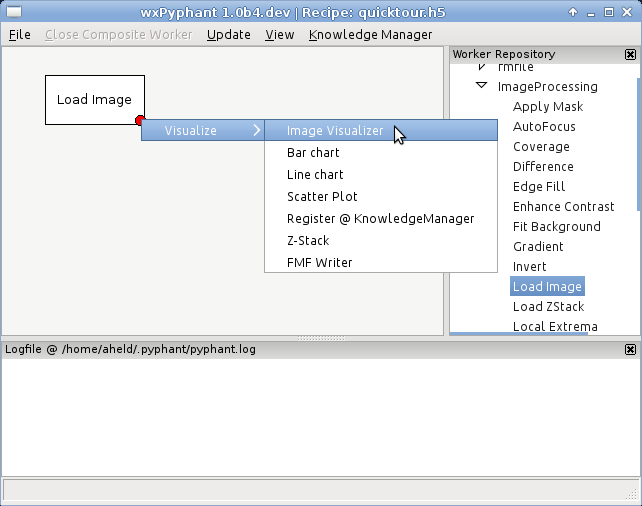
\includegraphics[scale=0.75]{fig/gui_context_menu.png}
  \caption{Visualizers are found by opening the context menu on a plug}
  \label{fig:gui_context_menu}
\end{figure}
The canonical choice for visualizing two dimensional |FieldContainers|
is the |Image Visualizer|. Selecting it will pop up a new window with
a false-color-visualization of the image data as in
\autoref{fig:gui_imagevis}.
\begin{figure}[h]
  \centering
  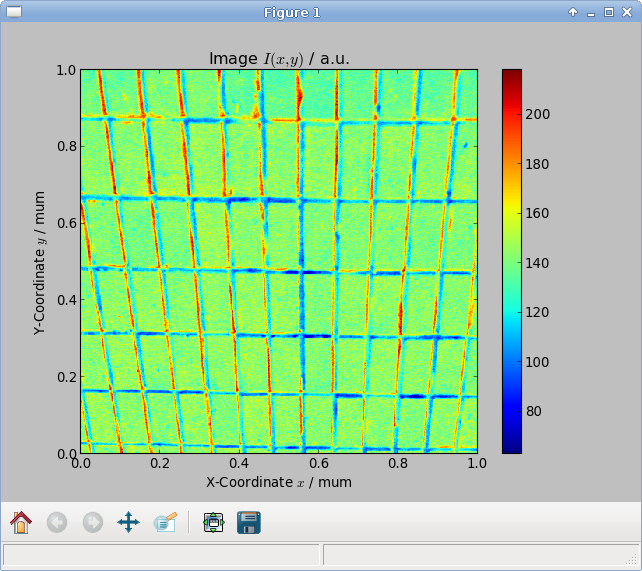
\includegraphics[scale=0.75]{fig/gui_imagevis.png}
  \caption{False-color visualization of a two dimensional FieldContainer}
  \label{fig:gui_imagevis}
\end{figure}
As some of the readers may have noticed, the |Image Visualizer| is
based on matplotlib\cite{matplotlib}. You may refer to matplotlib's
documentation on how to use the controls available in the toolbar of
the visualizer. As you can see in \autoref{fig:gui_imagevis}, the unit
of the field and the scalings of the axes are respected in the
visualization. If you want to choose another image, just go back and
edit the worker's |Filename| parameter until you are satisfied. We
have chosen a photography of a brick wall available for free
from~\url{http://sipi.usc.edu/database/}.

In a next step, we want to calculate the gradient magnitude of the
image we just imported. Pyphant already offers a worker for this
called |Gradient| also available in the |ImageProcessing|
toolbox. Please drag a |Gradient| worker into the recipe pane. As you
may have noticed, the |Gradient| worker not only offers a plug in
the bottom right corner but also a socket in the top left corner
indicated by a red square. In order to route the output from the |Load Image|
plug to the socket of the |Gradient| worker, simply connect
the two connectors by a drag and drop operation starting on the plug
and ending on the socket. The link should be visible as an
arrow similar as in \autoref{fig:gui_gradient_worker}.
\begin{figure}[h]
  \centering
  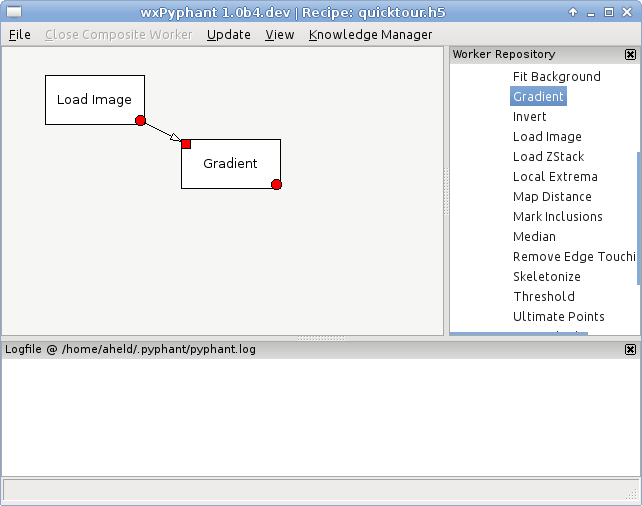
\includegraphics[scale=0.75]{fig/gui_gradient_worker.png}
  \caption{Information flow between workers is indicated by an
  arrow connecting the sockets}
  \label{fig:gui_gradient_worker}
\end{figure}
You may convince yourself that the |Gradient| worker offers no
parameters except for the possibility to rename it, which is always
available. As you have learned how to visualizing two dimensional
|FieldContainers| by now, you should be able to also visualize the
gradient magnitude. In \autoref{fig:gui_imagevis_gradient} we have shown
the visualizations of the original image and the gradient magnitude
side by side.
\begin{figure}[h]
  \centering
  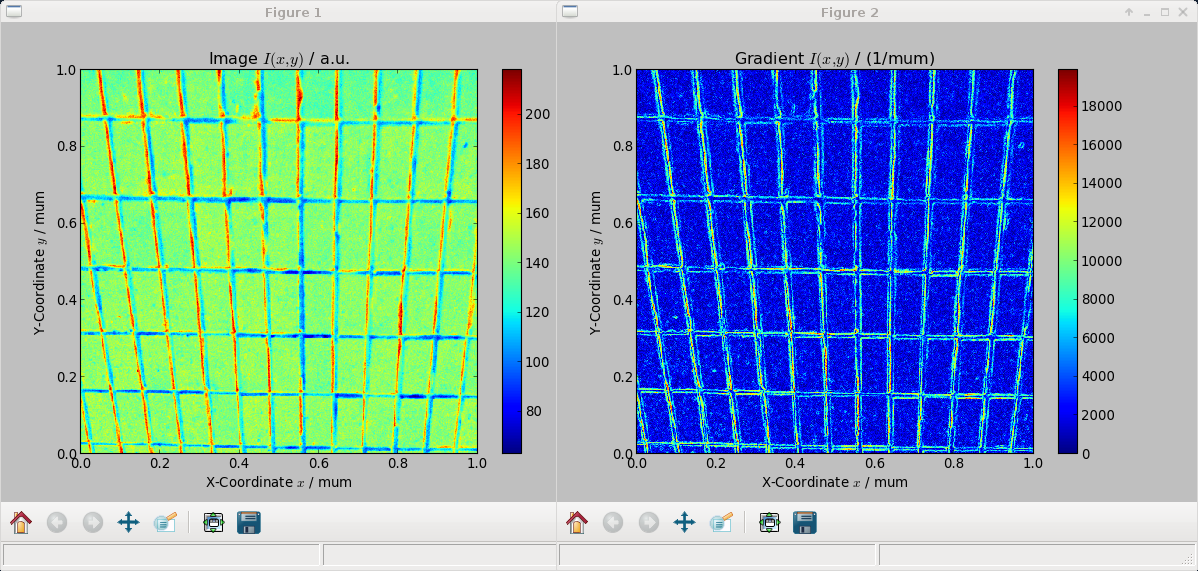
\includegraphics[width=\linewidth]{fig/gui_imagevis_gradient.png}
  \caption{Visualization of the original image (left) and its gradient
    magnitude (right)}
  \label{fig:gui_imagevis_gradient}
\end{figure}
Feel free to try the same on your recipe. Also note the correct
inference of the field unit of the gradient magnitude which is a first
order spatial derivative. The |Gradient| worker is unable to calculate
the gradient magnitude if the two axes of the original image are
incompatible. Try to set the axes units for instance to \si{m} and
\si{s}. You will get an error message and a python traceback will be
written to the log file which is also visible in the bottom of the
GUI. Go back and set both units to be compatible again.

In a last step, we add the |Histogram| worker from the |Statistics|
toolbox to the recipe. It takes a |FieldContainer| as input and
calculates a histogram of its field values as an output. In that case,
the output is a one dimensional |FieldContainer| irrespective of the
dimensionality of the input. You may want to set its |Bins| parameter
to a higher value than the default (10). Connect the |Gradient|
worker's output plug to the socket of the |Histogram| worker. Once
you're done with that, you can visualize the histogram by choosing the
|Bar chart| visualizer on the |Histogram| worker's plug which is
appropriate for histograms. If you are uncertain about those steps, go
back and review how we connected the |Gradient| worker and visualized
its output. In our case, the resulting visualization for 50 bins is
shown in \autoref{fig:gui_barvis_histo} as a reference. Your result
may differ depending on the image you have chosen, its scaling and the
number of bins you entered.
\begin{figure}[h]
  \centering
  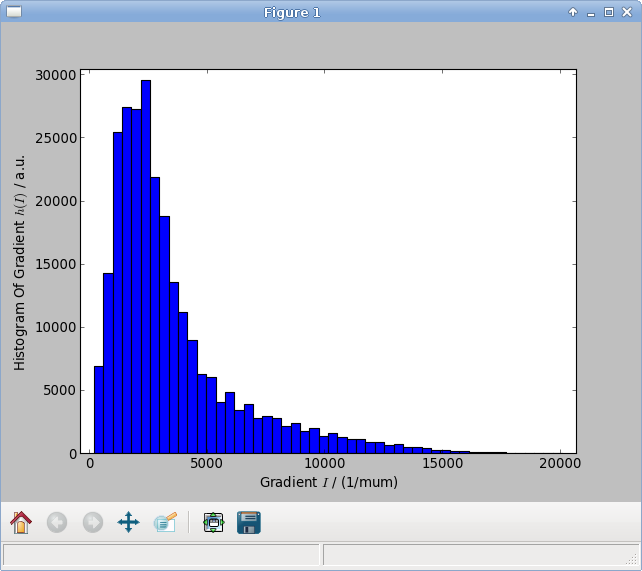
\includegraphics[scale=0.75]{fig/gui_barvis_histo.png}
  \caption{Bar chart visualization of a 50 bin histogram of the
    gradient magnitude}
  \label{fig:gui_barvis_histo}
\end{figure}

Having completed your first recipe, it is time to save it to
disk. The according menu items are found in the |File| menu. Also
notice the |Save results| checkbox in the |File| menu. It controls
whether the cached results of the workers should be saved to disk for
faster evaluation when reloading the recipe. You may uncheck it in
order to save disk space.

This completes the GUI part of the quick tour. In the next section, we
will learn how to write our own workers and visualizers and how to use
pyphant through its python API rather than through the GUI.

\FloatBarrier
\subsubsection{Extending and Scripting Pyphant}
\label{sec:introduction_extending_and_scripting}

For this part of the quick tour, we assume that the reader has a basic
knowledge of python\cite{python} and numpy\cite{numpy}. If this is not
the case, we recommend going through some of the tutorials to be found
on the respective homepages.

Let us begin by reformulating the above example by API calls instead
of graphical programming to get a first glimpse at pyphant's API:

\inputminted[linenos]{python}{api001.py}

As can be seen from the import statements in lines 2 -- 5, the
toolboxes shipped with pyphant are separate python packages. Usually,
a worker is located inside its own module, but this is not necessarily
the case. The core of pyphant is found in the |pyphant.core|
package. A recipe is also known as a |CompositeWorker| and an empty
one is created as shown in line 8. Every parameter of a worker is an
object. Paramters can be accessed by the magic (i.e. auto-generated)
attribute |param| followed by the name of the parameter, where the
first letter has to be capitalized. The value of a parameter is
accessed as shown in line 14.

Sockets and plugs can be accessed by name, but since all the workers
in our little example have at most one socket or plug, it is more
convenient to pick them as the only entry in the list of all sockets
or plugs as shown in line 20, which also illustrates how to connect a
plug and a socket. The result of a plug is obtained by calling
|getResult| on it. The underlying numpy array of a |FieldContainer| is
accessed as its |data| member. We have skipped the visualization of
the |FieldContainers| as we will come back to visualizers in a minute.

Also not shown is how to save the recipe to disk. IO in the HDF5
format is handled by the |pyphant.core.H5FileHandler.H5FileHandler|
class. Saving and loading a recipe is done as follows:

\inputminted[linenos]{python}{api002.py}

The |H5FileHandler| is used as a context manager similar to python's
builtin |open|. It supports the file modes |'r'|, |'w'| and |'a'|
which stand for read, (over)write and append respectively. When
loading a recipe, you may wonder how to access the workers contained
in it. For this purpose, every worker has a unique name, which happens
to also be a parameter called |Name|. The |Gradient| worker from the
GUI example could e.g. be accessed like so:

\inputminted[linenos]{python}{api003.py}

Now that we have covered how to assemble a recipe from existing
workers, it is time to learn how to implement a new worker. All
workers have to be derived from |pyphant.core.Worker.Worker|. A worker
consists of sockets, plugs and parameters. Let's look at an example on
how to specify those incredients. As a use case, we create a worker
that reads a |FieldContainer| and adds Gaussian noise to it with an
adjustable standard deviation:

\inputminted[linenos]{python}{api004.py}

Sockets are defined through the |_sockets| attribute which has to be a
list of 2-tuples. The first entry is the name of the socket and the
second entry is a data type hint. In our case, |TYPE_IMAGE| stands for
|FieldContainer|. Pyphant also supports |SampleContainers|, which are
tables where each column is a |FieldContainer|. The according data
type would then be |TYPE_ARRAY|. The somewhat strange naming of data
types has historic reasons and has never been changed since. There is
however no type checking performed by pyphant. The type hints are used
e.g. by the GUI to determine which visualizer is
appropriate. Connectors for |FieldContainers| will appear in red and
connectors for |SampleContainers| will appear in blue in the GUI as a
visual hint. So far we have defined a single socket named |"input_fc"|
which we expect to be a |FieldContainer|.

Similarly, parameters are defined as a list of 4-tuples. The entries
are the name, a label/short description (e.g. displayed in the parameter
dialog in the GUI), default value and a ``subtype'' hint for the GUI
dialog. In our case we define a parameter called |"width"| explained
to be the standard deviation with a default value of "1.0" and no
subtype hint. Again, no type checking is performed for parameters on
the API level. Only the GUI will guess a type from the default value
or use the subtype hint if provided (e.g. to show a file picker dialog
instead of a text box for a string default value). We have chosen a
string as the default value in order to also allow quantities with a
unit for the standard deviation.

Plugs are defined by applying the parametrized |plug| decorator which
expects a type hint as its single argument to a method. We want to
return a |FieldContainer|, so again we pass |TYPE_IMAGE| to the
decorator in line 14. The name of the decorated method defines the
name of the plug, in our case |"add_noise"|. Following the |self|
argument comes a list of arguments named like the sockets the result
of the plug depends on. The result of our plug depends on the single
socket |input_fc| and pyphant will automatically pass the result from
whatever plug is inserted into the |input_fc| socket into our
function. The last argument is used to keep track of the progress for
longer calculations and we can ignore it for now.

This covers all the boilerplate that is necessary for defining a
simple worker. Now we are left with the actual work of adding noise to
a |FieldContainer|. Remember that |FieldContainers| have a field
unit. The first thing we do is to calculate the standard deviation in
units of the input |FieldContainer|. For this purpose, we parse the
string value of the |width| parameter in line 16 with a helper
function from pyphant. The result is either a |float| or a
|pyphant.quantities.Quantity| object. The same applies to
|input_fc.unit|. When both units are compatible, the quotient
calculated in line 17 should be a |float|. We check this by trying to
cast to a |float| which would fail if the units of the standard
deviation and the input |FieldContainer| are incompatible. Then the
noisy data can be calculated with a standard numpy function, where we
also have to pass in the shape of the input data.

In a last step, we have to prepare the result as a
|FieldContainer|. For this purpose, we have to specify the data as a
numpy array which we just calculated. The field unit as well as the
dimensions are the same as from |input_fc|, so we copy them using
|deepcopy|. |FieldContainers| also have a longname and a
shortname/symbol. We append a hint to the original longname indicating
that noise has been added and we simply adopt the original symbol. No
deepcopy is necessary as strings/unicodes are immutable in
python. Additionaly, |FieldContainers| can have an assigned error and
mask which are also numpy arrays and user defined attributes which are
a python dictionary. We simply copy these from |input_fc|.

Before we return the resulting |FieldContainer|, we seal it by calling
its |seal| method. This ensures that no further changes can be made to
it and it also assignes a globally unique identifier to the
|FieldContainer|. See Reference~\cite{pyphant} for more details on
this subject.

In order to be able to try out our new worker inside pyphant's GUI, we
have to put it into a toolbox and tell pyphant about its
existence. This is done using the entry point mechanism from the
setuptools\cite{setuptools} package. Let's create a toolbox called
|quicktour|. First change the current working directory to wherever
you keep python sources:
\begin{minted}{bash}
$ cd $WhereEverYouKeepPythonSources
\end{minted}
Then create the file structure:
\begin{minted}{bash}
$ mkdir quicktour
$ cd quicktour
$ touch setup.py
$ mkdir quicktour
$ cd quicktour
$ touch __init__.py
$ touch addnoise.py
\end{minted}
Now paste the above code for the |Add Noise| worker into
|quicktour/quicktour/addnoise.py| and do the same for
\inputminted[linenos]{python}{api005.py}
and
\inputminted[linenos]{python}{api006.py}
This is a minimal example for
a toolbox. The important part is the |entry_points| argument to the
|setup| function. The entry point we are looking for is
|pyphant.workers|. The key of the entry is insignificant and the value
is a package that has a |workers| attribute. Our package is the
|quicktour| package and the |workers| attribute is defined in
|__init__.py|. The |workers| attribute is a list of module names which
should be imported by pyphant. Pyphant's GUI will then automatically
list any workers imported during this process. Let's try this out by
installing the toolbox. Please refer to the
setuptools~\cite{setuptools} documentation on how to install packages
on your system. Assuming you are inside a virtualenv or you have
configured setuptools to install to a local directory, this could be
done by calling
\begin{minted}{bash}
$ python setup.py develop
\end{minted}
inside the outer |quicktour| directory. The |develop| argument is
useful for changing the source code without the need to reinstall the
package. Once you are done, fire up the GUI and try out the new worker
as shown in Figures~\ref{fig:gui_addnoise_worker}
and~\ref{fig:gui_vis_noise}.
\begin{figure}[h]
  \centering
  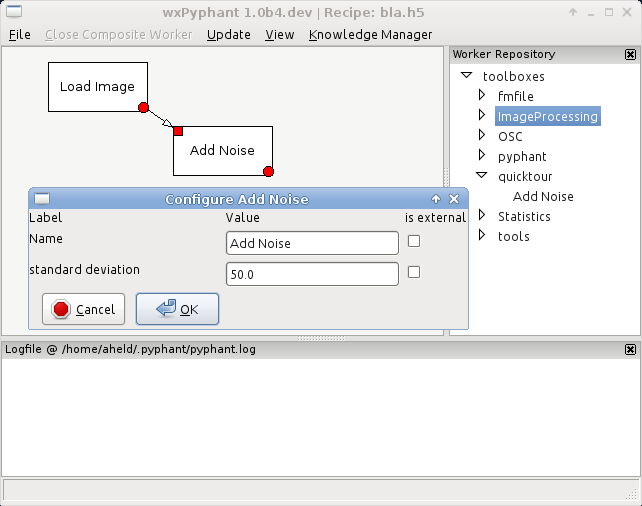
\includegraphics[scale=0.75]{fig/gui_addnoise_worker.png}
  \caption{The new toolbox and worker show up inside the GUI}
  \label{fig:gui_addnoise_worker}
\end{figure}
\begin{figure}[h]
  \centering
  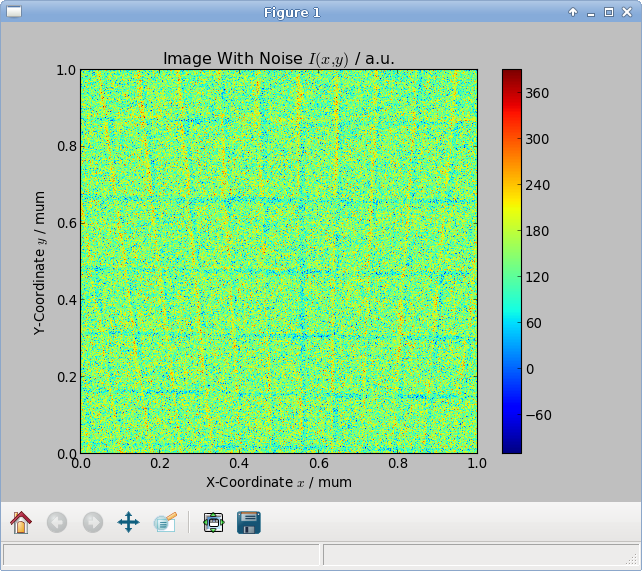
\includegraphics[scale=0.75]{fig/gui_vis_noise.png}
  \caption{False-color visualization of Gaussian noise added to a
    FieldContainer}
  \label{fig:gui_vis_noise}
\end{figure}

\FloatBarrier

As the last part of this quick tour, we write our own
visualizer. Assume you find the |Image Visualizer| just not fancy
enough and you want to have a height map surface plot instead. There
is no base class for visualizers in pyphant. Instead, a visualizer
may be defined by the following ``duck type'' interface:

\inputminted[linenos]{python}{api007.py}

So let's use matplotlib's\cite{matplotlib} |plot_surface| function for
our own visualizer, which we put inside the |quicktour| toolbox we
just created: \inputminted[linenos]{python}{api008.py} Visualizers
have to be registered as shown in lines 35--37. For this code to be
executed whenever we start the GUI, we abuse the worker import
mechanism, since pyphant does not provide a dedicated plugin system
for visualizers yet: \inputminted[linenos]{python}{api009.py} In order
to test the new visualizer, we first create a suitable
|FieldContainer| by smoothening our input image from
Figure~\ref{fig:gui_imagevis} with a median filter, calculating the
gradient magnitude, taking a threshold to extract the tile boundaries
and finally calculating a distance transform that assigns the shortest
distance to any tile boundary to every pixel. The recipe is shown in
Figure~\ref{fig:gui_use_surface_vis}. The parameters for the workers
to get a decent result depend on the input image and are not shown for
this reason. Try experimenting yourself with your image. The output of
the visualizer is shown in Figure~\ref{fig:gui_surface_vis}. As you
can see, we have not included any title, axes description, colormap
and so on. We leave this as an excercise to the reader and we end the
quick tour at this point.
\begin{figure}[h]
  \centering
  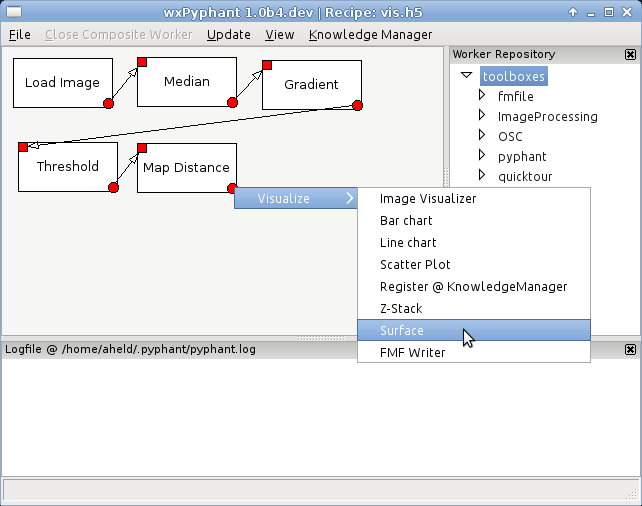
\includegraphics[scale=0.75]{fig/gui_use_surface_vis.png}
  \caption{Let's try out the new visualizer on a suitable example}
  \label{fig:gui_use_surface_vis}
\end{figure}
\begin{figure}[h]
  \centering
  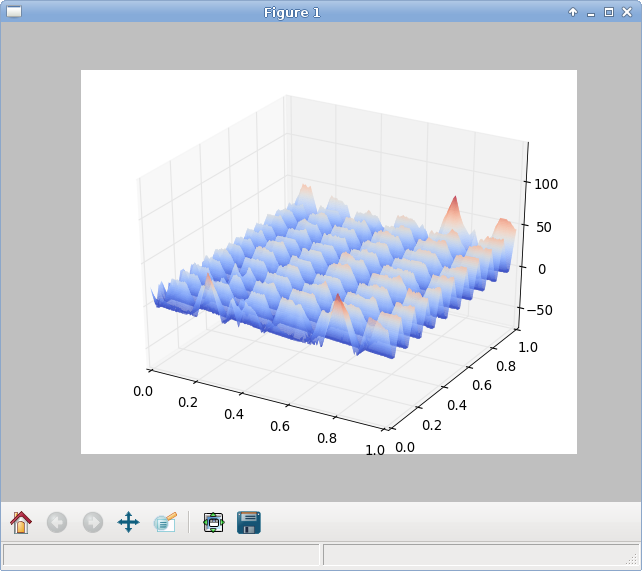
\includegraphics[scale=0.75]{fig/gui_surface_vis.png}
  \caption{First working version of the new visualizer}
  \label{fig:gui_surface_vis}
\end{figure}


\FloatBarrier
\section{Data Model}
\label{sec:data_model}

\subsection{Quantities}
\label{sec:data_model_quantities}

\subsection{Field Containers}
\label{sec:data_model_fcs}

\subsection{Sample Containers}
\label{sec:data_model_scs}

\subsection{Knowledge Manager}
\label{sec:data_model_knowledge_manager}

\section{Data Processing}
\label{sec:data_processing}

\subsection{Workers}
\label{sec:data_processing_workers}

\subsection{Recipes}
\label{sec:data_processing_recipes}

\subsection{Visualizers}
\label{sec:data_processing_visualizers}

\bibliographystyle{ieeetr}
\bibliography{bibliography}

\clearpage

\printindex

\end{document}

%%% Local Variables:
%%% TeX-PDF-mode: t
%%% End:
